\documentclass[aspectratio=169]{beamer}
%\documentclass{beamer}
\usetheme{Madrid}

\usepackage{graphicx}
\usepackage[utf8]{inputenc}
% Paquete para soporte de idioma español
\usepackage[spanish]{babel}
\usepackage{hyperref}
\usepackage{listings}
\usepackage{tikz}
\usetikzlibrary{positioning, arrows.meta, calc}

%\setbeamertemplate{footline}[frame number]

\begin{document}
	
	\title{Introducción a las redes neuronales}
	\subtitle{Redes neuronales recurrentes (RNN)}
	\author[J.I. Vasquez]{\textbf{Juan Irving Vásquez} \\jivg.org}
	\date{\today \copyright}
	\institute[jivg.org]{Centro de Innovación y Desarrollo Tecnológico en Cómputo \\ Instituto Politécnico Nacional}
	\titlegraphic{
\includegraphics[width=2cm]{ipn-cidetec}}
	
	\frame{\titlepage}
	
	
	\frame{
		\frametitle{Contenido}
		\tableofcontents
	}
	
	
	\section{Motivación}
	
	
	\begin{frame}
		\frametitle{Motivación}
		\begin{columns}
			\column{0.5\textwidth}
			\textbf{Datos Secuenciales}
			\begin{itemize}
				\item El orden importa. La salida actual depende del historial.
				\item Ejemplos:
				\begin{itemize}
					\item \textbf{Series de Tiempo:} Precios de acciones, datos climáticos.
					\item \textbf{Lenguaje (NLP):} Traducción, Análisis de Sentimientos.
					\item \textbf{Audio:} Reconocimiento de voz.
				\end{itemize}
			\end{itemize}
			
			\column{0.5\textwidth}
			\begin{figure}
				\centering
				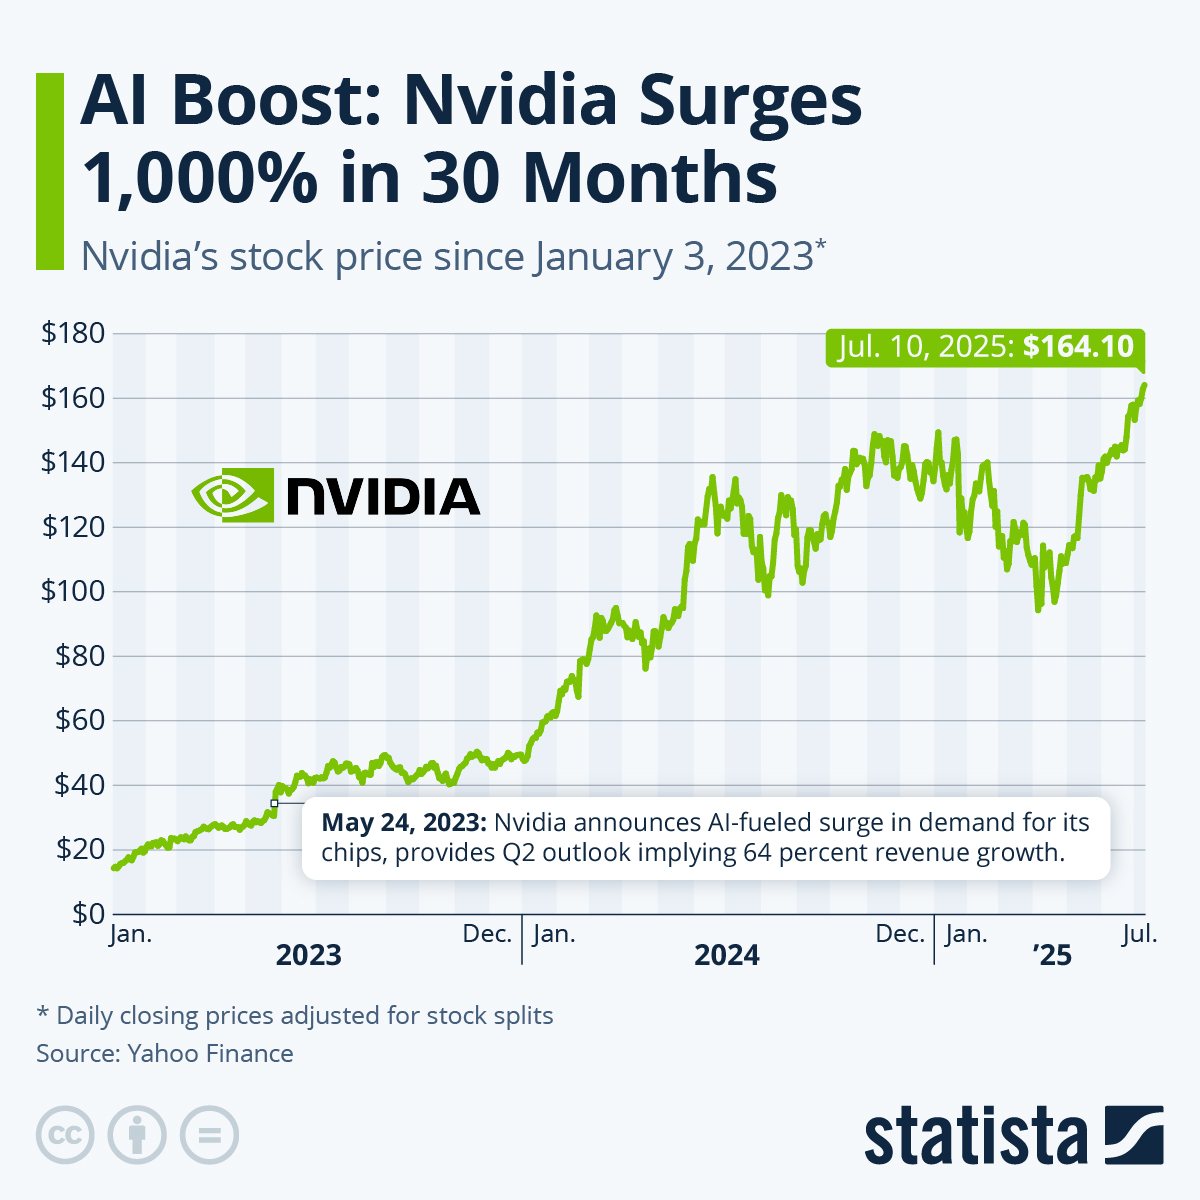
\includegraphics[height=0.65\textheight]{32358}
				\caption{Precios de acciones de Nvidia \footnote{\scriptsize https://www.statista.com/}}
				\label{fig:32358}
			\end{figure}
		\end{columns}
	\end{frame}
	
	
	
	\begin{frame}{Motivación}
		\framesubtitle{Uso de redes \textit{feed forward} en datos secuenciales}
		\begin{columns}
			\column{0.5\textwidth}
			\begin{itemize}
				\item Las redes \textit{feed forward} (FFN), por ejemplo, el perceptrón multicapa, tienen un tamaño de entrada fijo.
				\item Sin embargo, se pueden usar de la siguiente manera:
				\begin{itemize}
					\item Tamaño mayor que la entrada (se rellena la entrada / padding).
					\item Tamaño igual a la entrada (rara vez ocurre).
					\item Tamaño menor que la entrada (solo se analiza una sección).
				\end{itemize}
			\end{itemize}
			\column{0.5\textwidth}
			\begin{figure}
				\centering
				
\includegraphics[height=0.7\textheight]{input}
				\caption{Problema de entradas de tamaño diferente.}
				\label{fig:input}
			\end{figure}
		\end{columns}
	\end{frame}
	
	
	\begin{frame}
		\frametitle{Seq2seq con N-Gramas Neuronales}
		\framesubtitle{Ejemplo del uso de FFN en secuencias}
		\begin{center}
			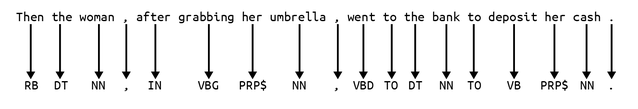
\includegraphics[height=0.25\textheight]{seq2seq}
		\end{center}
		
		\begin{center}
			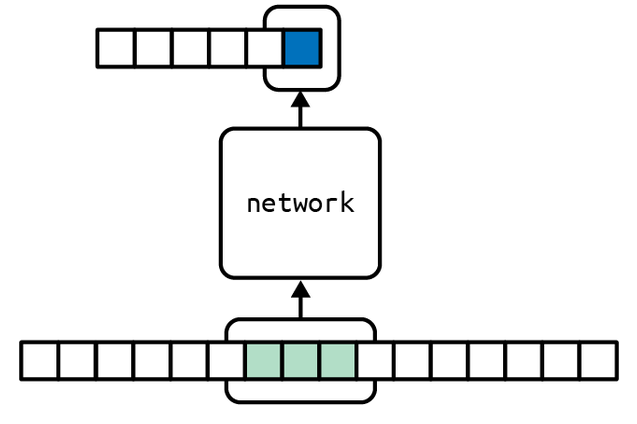
\includegraphics[height=0.5\textheight]{ngram}
		\end{center}
	\end{frame}
	
	\begin{frame}{Feedforward vs. recurrente}
		\begin{columns}
			\column{0.5\textwidth}
			\begin{itemize}
				\item Red neuronal feedforward (FNN)
				\begin{itemize}
					\item La información fluye en una sola dirección: \\ Entrada $\rightarrow$ Oculta $\rightarrow$ Salida.
				\end{itemize}
			\end{itemize}
			
			\vspace{0.5cm}
			
			\begin{itemize}
				\item Red neuronal recurrente (RNN). \\ Contiene un \textbf{bucle}. La salida de una neurona se retroalimenta a sí misma como entrada para el siguiente paso de tiempo.
				\begin{itemize}
					\item Mantiene un estado interno (memoria).
					\item Utiliza \textbf{Pesos Compartidos} en todos los pasos de tiempo.
				\end{itemize}
			\end{itemize}
			
			\column{0.5\textwidth}
			
			\begin{figure}
				\centering
				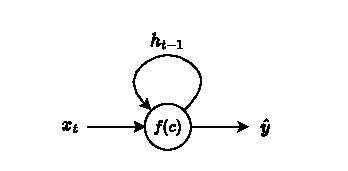
\includegraphics[width=\linewidth]{recurrent_nn.drawio}
				\caption{Nodo neuronal recurrente simple}
				\label{fig:recurrentnn}
			\end{figure}
		\end{columns}	
	\end{frame}
	
	
	\section{Red recurrente}
	
	
	\begin{frame}{La formulación matemática}
		En el paso de tiempo $t$, el estado oculto $h_t$ se actualiza utilizando la entrada $x_t$ y el estado oculto anterior $h_{t-1}$.
		
		\begin{equation}
			h_t = f(W_h h_{t-1} + W_x X_t + b)
		\end{equation}
		\textbf{Donde:}
		\begin{itemize}
			\item $h_t$: Nuevo estado oculto.
			\item $h_{t-1}$: Antiguo estado oculto (memoria del paso anterior).
			\item $X_t$: Vector de entrada actual.
			\item $W_h, W_x$: Matrices de pesos (Parámetros entrenables).
			\item $f(c)$: Función de activación.
		\end{itemize}
	\end{frame}
	
	
	\begin{frame}{Desenrollado a través del tiempo}
		Para entender las RNNs, las visualizamos como múltiples copias de la misma red, cada una pasando un mensaje a su sucesora.
		
		\vspace{1cm}
		
		\centering
		\begin{tikzpicture}[
			node distance=1.5cm,
			layer/.style={circle, draw, minimum size=1cm, fill=blue!10},
			arrow/.style={-Stealth, thick}
			]
			% Time step t-1
			\node[layer] (h_prev) {$h_{t-1}$};
			\node[below=of h_prev] (x_prev) {$x_{t-1}$};
			\node[above=of h_prev] (y_prev) {$y_{t-1}$};
			
			% Time step t
			\node[layer, right=of h_prev] (h_curr) {$h_t$};
			\node[below=of h_curr] (x_curr) {$x_t$};
			\node[above=of h_curr] (y_curr) {$y_t$};
			
			% Time step t+1
			\node[layer, right=of h_curr] (h_next) {$h_{t+1}$};
			\node[below=of h_next] (x_next) {$x_{t+1}$};
			\node[above=of h_next] (y_next) {$y_{t+1}$};
			
			% Connections
			\draw[arrow] (x_prev) -- (h_prev);
			\draw[arrow] (h_prev) -- (y_prev);
			
			\draw[arrow] (x_curr) -- (h_curr);
			\draw[arrow] (h_curr) -- (y_curr);
			
			\draw[arrow] (x_next) -- (h_next);
			\draw[arrow] (h_next) -- (y_next);
			
			% Recurrent connections
			\draw[arrow] (h_prev) -- node[above] {$W_h$} (h_curr);
			\draw[arrow] (h_curr) -- node[above] {$W_h$} (h_next);
			
			% Ellipsis
			\node[left=of h_prev] (start) {$\dots$};
			\draw[arrow] (start) -- (h_prev);
			\node[right=of h_next] (end) {$\dots$};
			\draw[arrow] (h_next) -- (end);
			
		\end{tikzpicture}
	\end{frame}
	
	
	
	%\begin{frame}
	%	\frametitle{Recurrent network}
	%	\begin{center}
		%		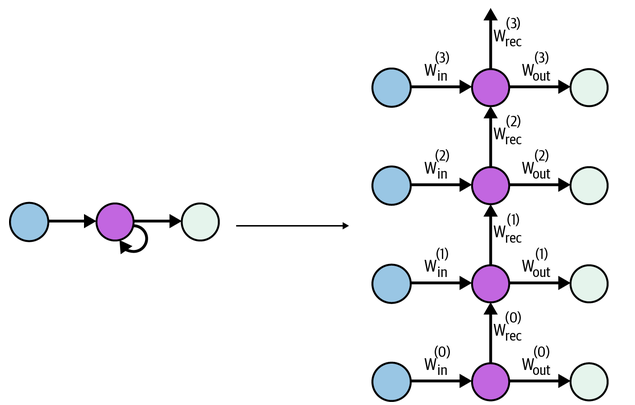
\includegraphics[height=0.6\textheight]{recurrent one}
		%	\end{center}	
	%	\begin{equation}
		%		f^t = f(w_{in} x^{(t)} + w_{rec} f^{(t-1)} )
		%	\end{equation}
	%\end{frame}
	
	
	
	
	%\begin{frame}
	%	\frametitle{Recurrent networks}
	%	\begin{center}
		%		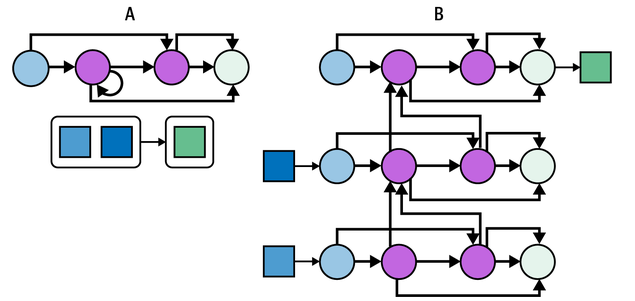
\includegraphics[height=0.6\textheight]{extendido}
		%	\end{center}
	%\end{frame}
	%
	
	
	%
	%\begin{frame}
	%	\frametitle{title}
	%\end{frame}
	
	
	
	% =========================================================================
	\section{Entrenamiento y Desafíos}
	% =========================================================================
	
	\begin{frame}{Retropropagación a través del tiempo (BPTT)}
		\begin{itemize}
			\item El entrenamiento es similar al Backpropagation estándar, pero los gradientes fluyen hacia atrás a través del tiempo.
			\begin{enumerate}
				\item Se hace inferencia frontal.
					$$[h_1, \dots, h_n] = \Phi([x_1,\dots,x_n])$$
					$$\hat{y} = h_n$$
				\item Comparamos la secuencia predicha con la secuencia objetivo para calcular la Pérdida.
				$$ L(y, \hat{y})$$
				\item Calculamos $\frac{\partial L}{\partial W}$ para cada tiempo. 
				\item Sumamos los gradientes para todos los instantes de tiempo.
				\item Actualizamos los pesos con el acumulado de gradientes.
			\end{enumerate}
		\end{itemize}
		
	\end{frame}
	
	
	\frame{
		\frametitle{Implementación de Backpropagation}
		\begin{itemize}
			\item En la capa de salida tienes el error en el tiempo $T$ (último tiempo),
			\item Podemos generalizar el término de error anterior como $\delta_t$,
			\item Término de error para el nodo de la capa oculta $t$,
			\begin{equation}
				\delta_t = w_{h} \delta_{t+1} f'(c_t),
			\end{equation} donde $c$ es la combinación lineal
			\item El incremento se calcula por tiempo,
			\begin{equation}
				\Delta w_{x|t} = \eta \delta_t x_{i}
			\end{equation}
			\begin{equation}
				\Delta w_{h|t} = \eta \delta_t h_{i}
			\end{equation}
			\begin{equation}
				\Delta b{t} = \eta \delta_t (1)
			\end{equation}
		\end{itemize}
	}
	
	
	
	\begin{frame}{El problema del desvanecimiento del gradiente}
		\textbf{El Problema:}
		\begin{itemize}
			\item Dado que la misma matriz $W$ se multiplica repetidamente (regla de la cadena) durante la retropropagación.
			\item Si los pesos son pequeños ($<1$), los gradientes se reducen exponencialmente $\rightarrow$ \textbf{Desvanecimiento del Gradiente}.
			\item Si los pesos son grandes ($>1$), los gradientes crecen exponencialmente $\rightarrow$ \textbf{Explosión del Gradiente}.
		\end{itemize}
		\begin{alertblock}{Consecuencia}
			La red deja de aprender de las entradas tempranas en secuencias largas. \\ Sufre de \textbf{Memoria a corto plazo}.
		\end{alertblock}
		\textbf{Ejemplo:}
		\begin{quote}
			"Crecí en \textbf{Francia}... [párrafo largo] ... Hablo \textbf{francés} fluido."
		\end{quote}
		
		Una RNN con desvanecimiento de gradientes podría olvidar el contexto "Francia" para cuando necesite predecir "francés".
	\end{frame}
	
	% =========================================================================
	\section{Extensiones: LSTM y GRU}
	% =========================================================================
	
	\begin{frame}{Solución: memoria a corto y largo plazo (LSTM)}
		Introducida por Hochreiter \& Schmidhuber en 1997\footnote{\scriptsize Hochreiter, S., \& Schmidhuber, J. (1997). Long short-term memory. Neural computation, 9(8), 1735-1780.}.
		\begin{columns}
			\column{0.5\textwidth}
			\begin{itemize}
				\item Introduce un \textbf{estado de celda} ($C_t$) que actúa como una autopista de información.
				\item Utiliza \textbf{compuertas} para regular el flujo de información:
				\begin{enumerate}
					\item \textbf{Compuerta de olvido:} \\¿Qué eliminar de la memoria?
					\item \textbf{Compuerta de entrada:}\\ ¿Qué nueva información almacenar?
					\item \textbf{Compuerta de salida:}\\ ¿Qué mostrar como salida?
				\end{enumerate}
			\end{itemize}
			\column{0.5\textwidth}
			\begin{figure}
				\centering
				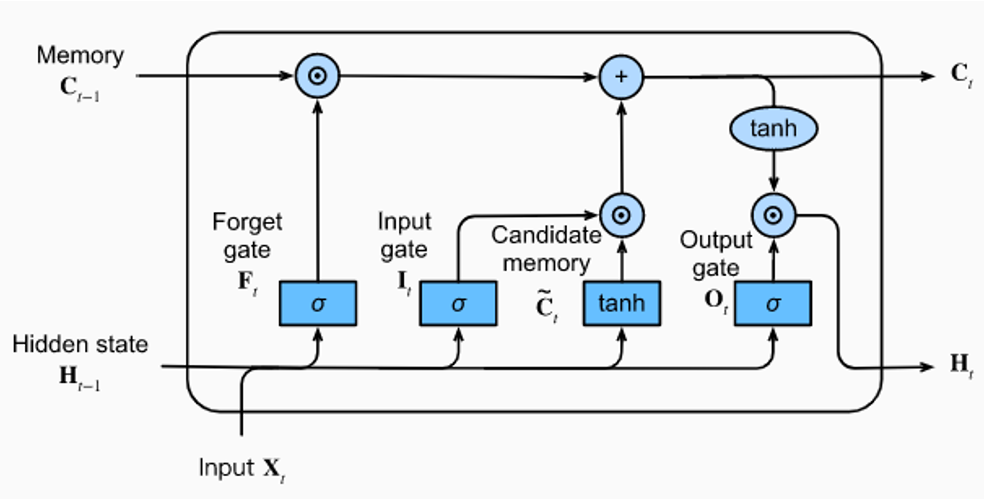
\includegraphics[width=\linewidth]{1_Mb_L_slY9rjMr8-IADHvwg}
				\caption{Red neuronal LSTM}
				\label{fig:1mblsly9rjmr8-iadhvwg}
			\end{figure}
		\end{columns}
	\end{frame}
	
	
	\begin{frame}{Alternativa: unidad recurrente con compuertas (GRU)}
		Introducida por Cho et al., en 2014\footnote{\scriptsize Cho, K., Van Merriënboer, B., Gulcehre, C., Bahdanau, D., Bougares, F., Schwenk, H. and Bengio, Y., 2014. Learning phrase representations using RNN encoder-decoder for statistical machine translation. arXiv preprint arXiv:1406.1078.}.
		\begin{columns}
			\column{0.5\textwidth}
			\begin{itemize}
				\item Una versión simplificada de LSTM.
				\item Fusiona el estado de la celda y el estado oculto.
				\item Combina las compuertas de olvido y entrada en una sola \textbf{compuerta de actualización}.
				\item \textbf{Beneficio:} menos parámetros, más rápida de entrenar, a menudo funciona igual de bien.
			\end{itemize}
			
			\column{0.5\textwidth}		
			\begin{figure}
				\centering
				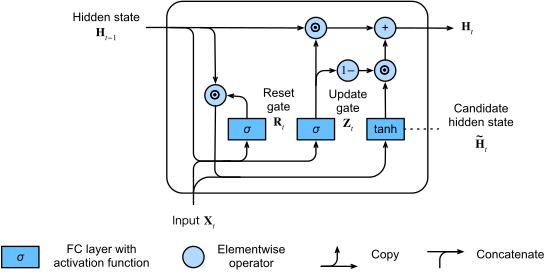
\includegraphics[width=\linewidth]{gru-3}
				\caption{Red neuronal GRU}
				\label{fig:gru-3}
			\end{figure}
		\end{columns}
	\end{frame}
	
	% =========================================================================
	\section{Conclusión}
	% =========================================================================
	
	\begin{frame}{Resumen}
		\begin{itemize}
			\item Las \textbf{RNNs} están diseñadas para datos secuenciales donde el historial importa.
			\item Comparten pesos a través de los pasos de tiempo ($W_h, W_x$).
			\item El entrenamiento se realiza mediante \textbf{Retropropagación a través del tiempo (BPTT)}.
			\item El \textbf{desvanecimiento de gradientes} hace que las RNNs estándar sean difíciles de entrenar en secuencias largas.
			\item Las \textbf{LSTMs y GRUs} resuelven esto utilizando mecanismos de compuertas para preservar dependencias a largo plazo.
		\end{itemize}
	\end{frame}
	
	
	\begin{frame}
		\frametitle{Referencias}
		\begin{itemize}
			\item Du, K.L. and Swamy, M.N., 2013. Neural networks and statistical learning. Springer Science \& Business Media.
			\item Zhang, A., Lipton, Z.C., Li, M. and Smola, A.J., 2023. Dive into deep learning. Cambridge University Press.
			\item Goodfellow, Ian, Yoshua Bengio, and Aaron Courville. Deep learning. MIT press, 2016.
			\item NYU, Aprendizaje profundo, \url{https://atcold.github.io/pytorch-Deep-Learning/es/week07/07-3/}
		\end{itemize}
	\end{frame}
	
	
\end{document}